\documentclass{article}

% If you need to pass options to natbib, use, e.g.:
%     \PassOptionsToPackage{numbers, compress}{natbib}
% before loading neurips_2020

% ready for submission
% \usepackage{neurips_2020}

% to compile a preprint version, e.g., for submission to arXiv, add the
% [preprint] option:
%     \usepackage[preprint]{neurips_2020}

% To compile a camera-ready version, add the [final] option, e.g.:
%     \usepackage[final]{neurips_2020}

% To avoid loading the natbib package, add option nonatbib:
\usepackage[nonatbib, final]{neurips_2020}

\usepackage[utf8]{inputenc} % allow utf-8 input
\usepackage[T1]{fontenc}    % use 8-bit T1 fonts
\usepackage{hyperref}       % hyperlinks
\usepackage{url}            % simple URL typesetting
\usepackage{booktabs}       % professional-quality tables
\usepackage{amsfonts}       % blackboard math symbols
\usepackage{nicefrac}       % compact symbols for 1/2, etc.
\usepackage{microtype}      % microtypography
\usepackage{amsmath}
\usepackage[pdftex]{graphicx}
\usepackage[table]{xcolor}
\usepackage{caption}
\usepackage{subcaption}
\usepackage{multicol}
\usepackage{multirow}
\usepackage{algorithm}
\usepackage{algpseudocode}

\bibliographystyle{unsrturl}

\title{Compressed CNNs for Cover Song Identification}

% The \author macro works with any number of authors. There are two commands
% used to separate the names and addresses of multiple authors: \And and \AND.
%
% Using \And between authors leaves it to LaTeX to determine where to break the
% lines. Using \AND forces a line break at that point. So, if LaTeX puts 3 of 4
% authors' names on the first line, and the last on the second line, try using
% \AND instead of \And before the third author name.

\author{%
  Vivian~Li \\
  vdl21 \\
}

\begin{document}

\maketitle

\begin{abstract}
    With the internet continually evolving toward multimedia-based searches and information retrieval, audio content identification is becoming evermore important. Related to this problem is the challenge of cover song identification, seeking to identify similar songs despite considerable differences in tempo, pitch, and structure. In this paper, I train several deep convolutional neural networks to perform cover song identification, looking to optimise such models for mobile deployment. Evaluating these networks on datasets of classical and pop music, I look to investigate the effects of compression on classification accuracy and inference speed, informing the development of efficient and accurate music information retrieval models for mobile devices.
\end{abstract}

\section{Introduction}\label{sec:introduction}
% An articulated umbrella objective and purpose for the project, that is carefully broken down into a series of interrelated sub-questions that build towards the objective. If necessary, more than just one hypothesis is included. 

Since the early 2000s, with the development of efficient music fingerprinting methods like Shazam \cite{Shazam}, compact forms of music recognition have been an ongoing topic of research \cite{Six2014, Baluja2008, Ramona2013, Sonnleitner2016}. However, such research has mostly been in the field of music fingerprinting, the process of matching an incoming sound \textit{query} with a database of \textit{reference} songs. However, fingerprinting techniques have struggled to generalise to more complicated forms of songs like classical music, where the musical interpretations of each performer introduce musical variations in tempo, expressive timings, instrumentation, and other musical aspects beyond the capabilities of most fingerprinting methods \cite{Arzt2017}. As such, the new task of cover song identification has emerged more recently, aiming to identify ``cover songs,'' i.e. adaptations of an original song. This research also has broader applications beyond simple song identification, as the similarity metrics used in such research can also help recommendation algorithms find similar music (e.g., Spotify), or copyright detection software find infringing songs (e.g., YouTube Content ID).

In this paper, I implement multiple convolutional neural networks (CNNs) to detect cover songs and apply them to identify performances of classical pieces. Aiming to adapt cover song identification for mobile deployment, I test the impact of several compression methods, including pruning and quantisation, on the model's performance and inference speed. To assess possible applications of these CNNs for mobile and embedded devices, I further compare the reduced model sizes in the context of microprocessor memory requirements.

\section{Related Work}\label{sec:related}
% Adequate (but not excessive) motivation and background information so that the reader has enough content to understand the reasons for, and importance of, the exploration and work performed. Crisp arguments motivate not only the objectives but also potential resulting findings and observations. The space given in the report to this type of content should not be excessive, and leave plenty of room for reporting and describing the technical work and thinking that forms the core of the project.
% Where necessary, relationships are drawn with prior knowledge and the text in the report bridges between what is sought in the project and what is already known. The project is placed in the context of prior and current ongoing research or conventional practice/wisdom.

The amount of research in cover song identification is extensive, with the best models competing in conferences like MIREX\footnote{\href{https://www.music-ir.org/mirex/wiki/MIREX\_HOME}{https://www.music-ir.org/mirex/wiki/MIREX\_HOME}} Existing research has already obtained significant results through both deep learning and traditional approaches. Widmer et. al. \cite{Arzt2017} develop an adaptation of fingerprinting for classical music identification through an automatically compiled reference database. However, the use of fingerprinting leads to a large reference database, making this method unsuitable for mobile deployment. The system was also only tested on classical piano music. Rein et. al. \cite{Rein2006} introduce a more traditional method of identifying classical music compositions using a combination of \textit{wavelet dispersion vectors} as characteristic features and a simple two-layer neural net. In addition to this, more deep learning approaches have also been applied, with Siamese CNNs \cite{Varior2016} used for live song identification \cite{Hakala2023} and CNNs used to extract latent representations for similarity comparison \cite{Xu2018}. This work builds off of existing work on cover song identification using CNNs by Yu et. al. \cite{Yu2020}, aiming to adapt it for mobile deployment.

\section{Background}\label{sec:background}
% Convincing technical depth and solid fundamental understanding of techniques, algorithms and concepts used are provided. These are scoped based on relevance to the project. Limitations of these tools/techniques are appreciated and included in thinking and writing, relationships to well-known mainstream related techniques are acknowledged, as are very closely related work (if applicable).

\subsection{Digital Signal Processing}\label{sec:dsp}
The use of Fourier transforms is widespread throughout engineering and computer science. As the Fourier transform decomposes a time signal into its frequency components, the short-time Fourier transform can be used to track how those frequency components change over time, exposing important features like pitch and tempo for musical analysis.

However, the Fourier transform divides its output bins equally in frequency space. For musical applications, musical notes are situated logarithmically in frequency space, with one octave (7 notes) doubling in frequency. Consequently, the Fourier transform ends up under-sampling higher musical notes (Figure \ref{fig:cqt-comparison}). Thus, musical applications often use the \textbf{constant-Q transform} (CQT), which adapts the short-time Fourier transform to be logarithmically spaced in frequency.
\begin{figure}[h]
    \centering
    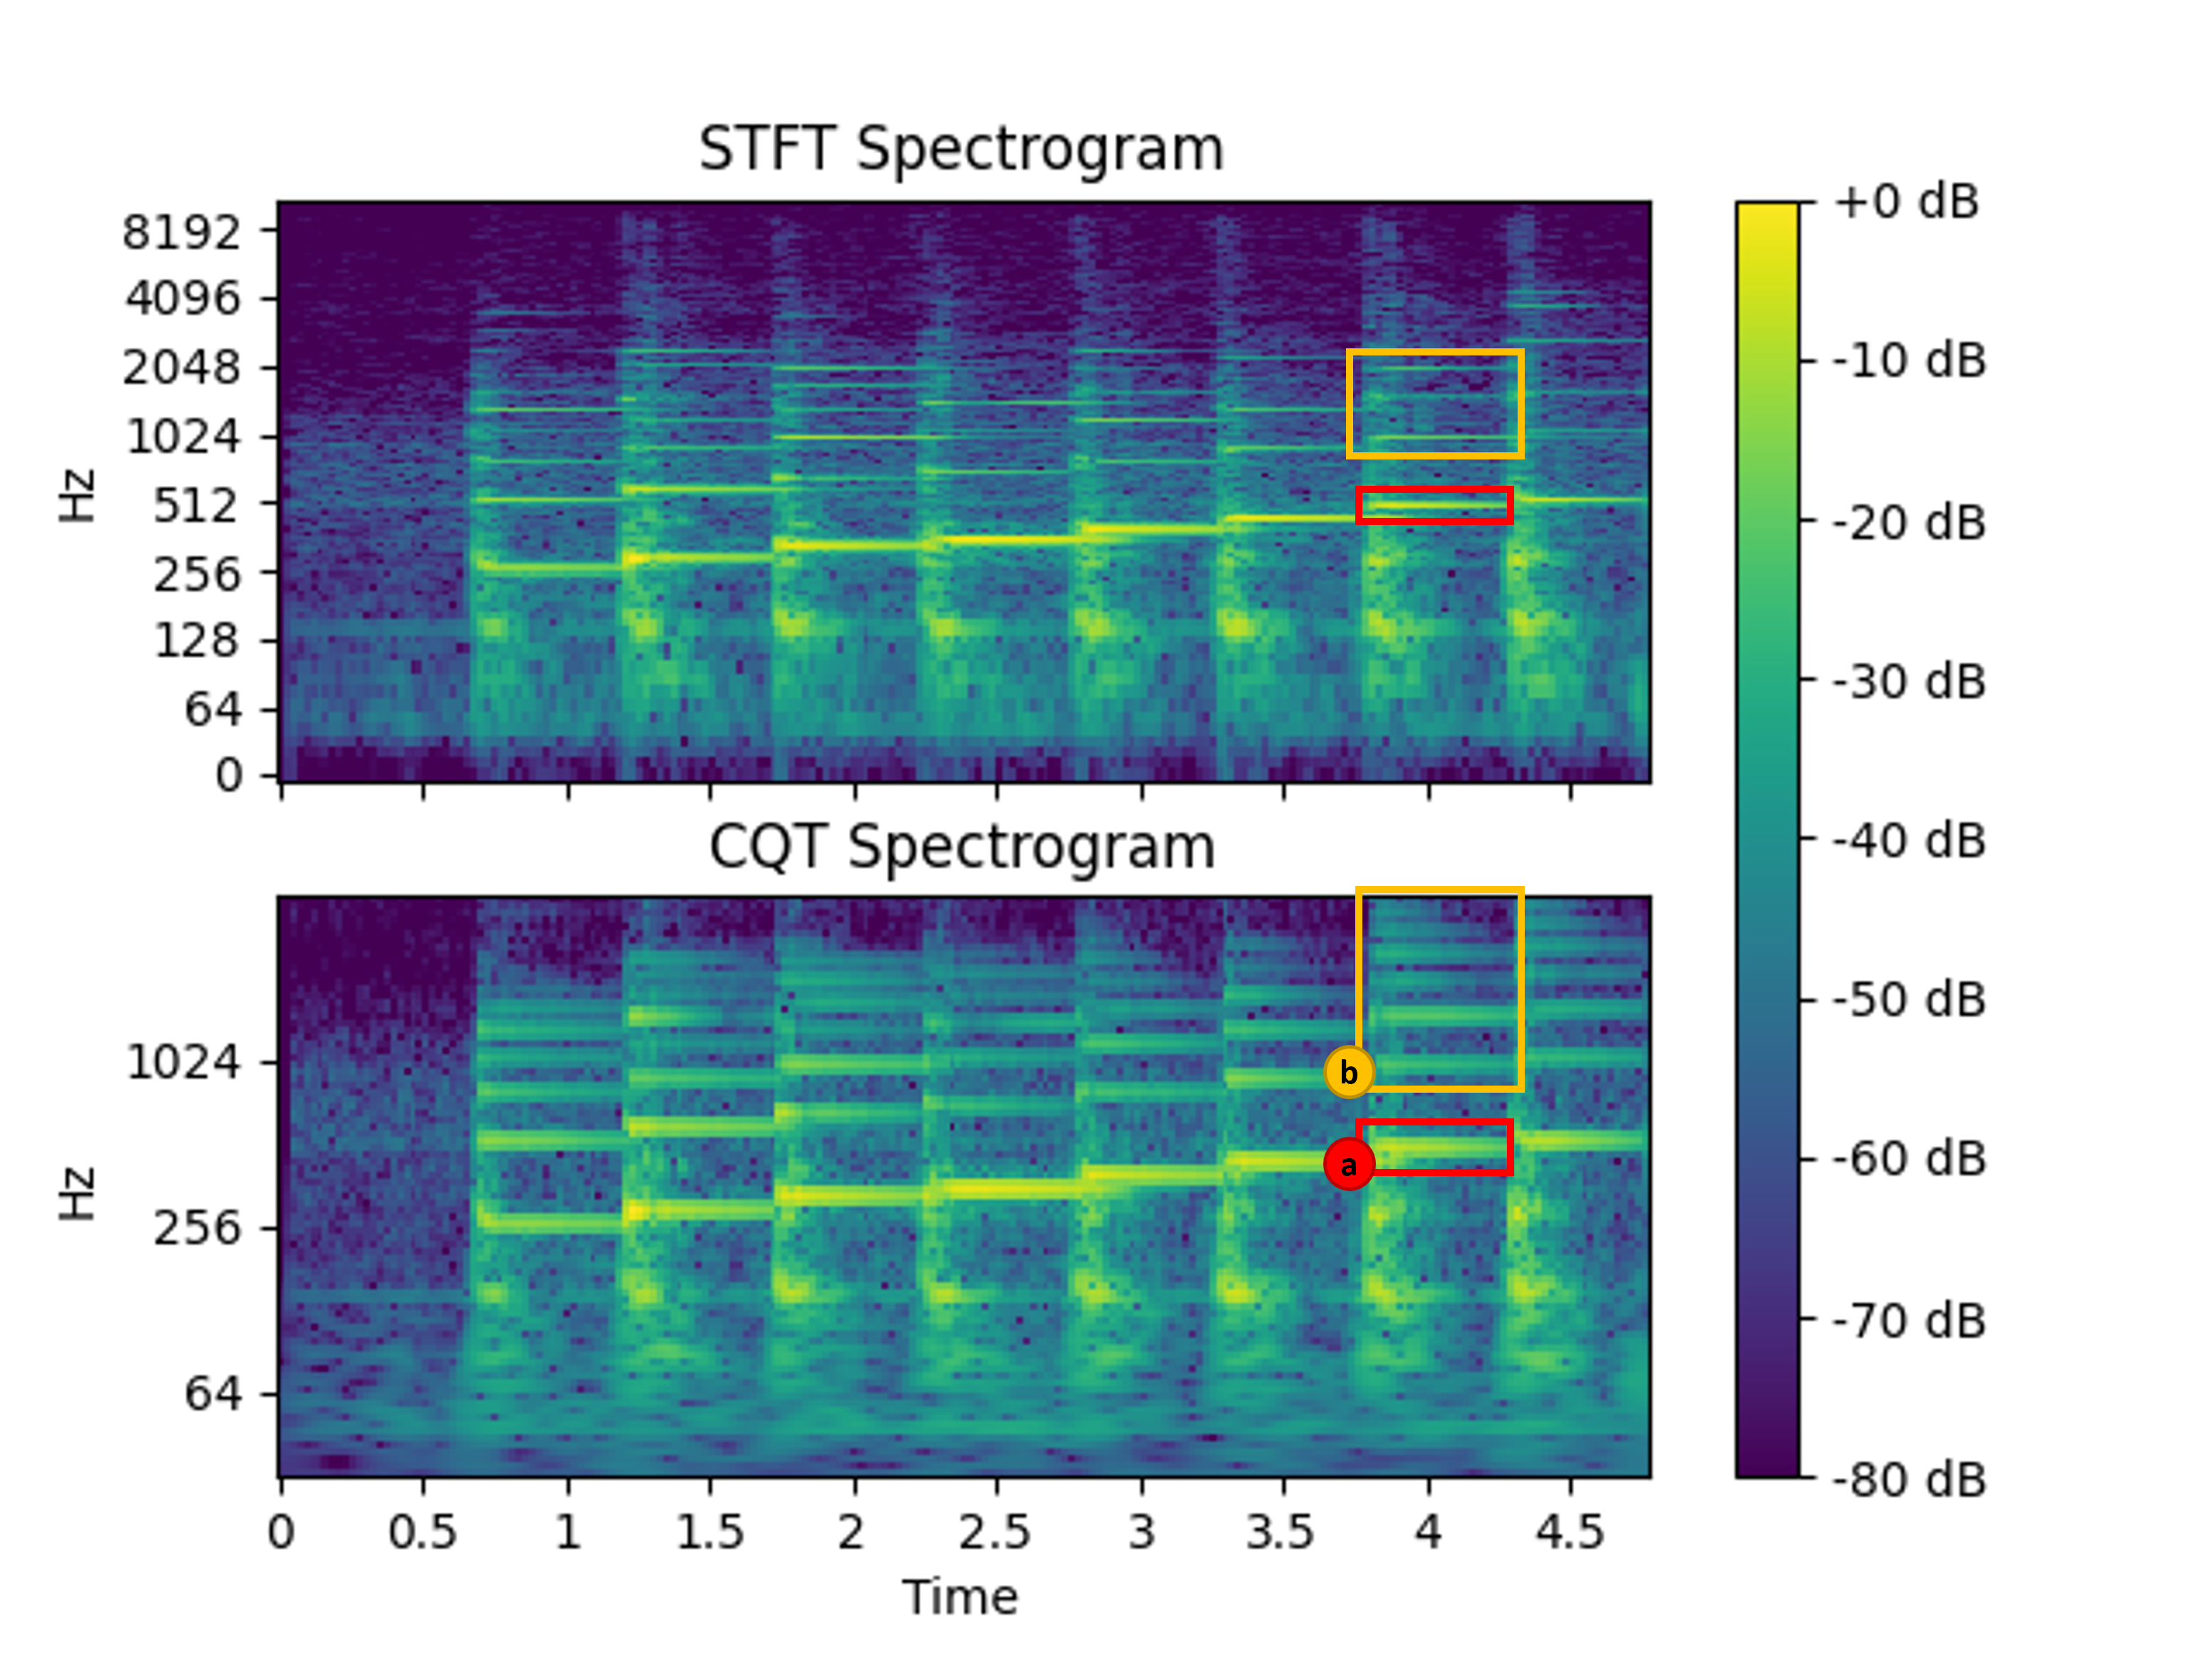
\includegraphics[width=0.9\textwidth]{figures/spectrogram_comparison_final.png}
    \caption{STFT and CQT spectrograms of a C-major piano scale. (a) CQT has even-thickness fundamental frequency bands. (b) STFT harmonics disappear at higher frequencies.}
    \label{fig:cqt-comparison}
\end{figure}

\subsection{Model Compression}\label{sec:compression}
To design a system capable of real-time performance on a mobile device, I explore three different optimisation techniques for minimising model size and inference latency. In Section \ref{sec:evalcomp}, I look at the impact of these techniques on inference time and accuracy.

\subsubsection{Depthwise Separable Convolution}\label{sec:dwpcnn}
% https://openreview.net/pdf?id=S1jBcueAb#:~:text=Depthwise%20separable%20convolutions%20are%20strictly,cheaper%20to%20train%20and%20run.
Depthwise separable convolutions are a method of reducing the size of individual convolutional layers in a CNN by splitting the convolution into smaller depthwise and separable convolutions.

Instead of defining a kernel that operates over all input channels to the layer (e.g., 3 x 3 x 3), a depthwise convolution layer instead separates this kernel into smaller separate kernels applied to each channel independently (e.g., 3 x 3 x 1), forming distinct intermediate layers. The outputs of these depth-wise convolutions are then combined with a separable convolution (i.e., a point-wise convolution) to introduce dependencies between the different layers (Figure \ref{fig:dwscnn}).
\begin{figure}[h]
    \centering
    \includegraphics[width=0.95\textwidth]{figures/cnn_diagram_final.png}
    \caption{A comparison between CNNs and Depthwise Separable CNNs}
    \label{fig:dwscnn}
\end{figure}

By replacing convolutional layers with depthwise separable convolutions, we obtain a smaller and more efficient network, while maintaining information across the input channels \cite{Chollet2017}.

\subsubsection{Pruning}\label{sec:pruning}
Pruning is a method of model compression by systematically removing certain parameters or even entire neurons. Pruning operates on the sparse network assumption that a large majority of network weights will have little impact on the model's predictions. Thus, by pruning these low-impact weights, we obtain a smaller network with performance comparable to the original.

For more effective pruning, it is more beneficial to prune after the model has been optimised, such that parameter weights can be taken as a measure of importance. As such, I choose to prune iteratively from an initial trained model, switching between tuning the network for some number of epochs and pruning more parameters.

\subsubsection{Weight Quantisation}\label{sec:quantization}
Quantisation is another method of model compression by changing the bit-width of the data structures used to store the model parameters. This reduction reduces the model's size, but can also make the model's inference quicker. Additionally, the most common form of quantisation, integer quantisation, which I implement in this paper, also allows the model to take advantage of existing hardware optimisations for integers.

Quantisation is most commonly done after training (i.e., training a model with float32 weights, then quantising to uint8), which I implement through TensorFlowLite \cite{Demosthenous2021}.

\section{Methods}\label{sec:methods}
% A sound systematic methodology is employed. Where possible it builds on methods seen in the literature or deviates from these when there is a reason to do so and discusses the reasons why. The steps within this method align well with the objectives of the project. If required, baseline methods that act as a point of comparison are offered and included in the discussion of results. Awareness of the impact of certain datasets or baselines (if applicable) not being included in a method is acknowledged. 
\subsection{Dataset}\label{sec:dataset}
Considering the primary focus of this paper towards classical music identification, I decided to use a collection of classical pieces from RondoDB \cite{RondoDB} as my training dataset. This dataset consists of 100 different classical pieces from a variety of composers and a multitude of instruments, with 5 recordings for each piece. For evaluation, the datasets used follow the literature, with the Mazurkas dataset \cite{MazurkaProject} used to evaluate performance on classical pieces and the Covers80 \cite{Covers80} dataset used to evaluate the system's generalizability to popular music. The Mazurkas dataset consists of 49 different classical piano pieces (Mazurkas composed by Frédéric Chopin) with over 10 performers for each piece. The Covers80 dataset consists of 80 pop songs, containing one original recording and one cover for each. While the recordings for the Covers80 dataset are available outright, the recordings for the RondoDB and Mazurkas datasets were obtained by scraping through YouTube\footnote{using \href{https://github.com/ytdl-org/youtube-dl}{\textbf{youtube-dl}}}, taking the first matching result.

These recordings were averaged to a single channel and resampled to 22050 Hz, before being converted to CQTs using Librosa \cite{McFee2015}, using 12 bins per octave and a Hann window with a hop length of 512.

For training, the CQTs were further augmented to improve the model's capability to generalise (Algorithm \ref{alg:trainingcqt}). For a given batch of recordings, each recording was first converted into a CQT, and then compressed with a mean filter and down-sampled by 20 times. Then, tempo changes were simulated by stretching the CQT by a random changing factor $r$ chosen uniformly between 0.7 and 1.3. Because most deep learning frameworks like TensorFlow require fixed-dimensional batched inputs, the entire batch of processed CQTs was then cropped to a length of either 200, 300, or 400 samples.

\begin{algorithm}
    \caption{Training data augmentation}
    \label{alg:trainingcqt}
    \begin{algorithmic}
        \Require $l\in \{200, 300, 400\}$
        \Ensure $B$ is a batch of recordings in dataset $D$
        \For{$x$ in $B$}
            \State $r \gets \mathcal{U}(0.7, 1.3)$
            \State $X \gets \mathbf{CQT}(x)$
            \State $X \gets$ stretch/squash by $r$
            \State $X \gets$ crop random subsequence of length $l$
        \EndFor
    \end{algorithmic}
\end{algorithm}

\subsection{Models}\label{sec:models}
% A description of the implementation developed and/or used within the project as part of the methodology. This should not be overly verbose but still explain sufficiently to indicate various frameworks and open-source software used. This content ties to the experiment discussion and helps explain how the experiments were performed. 
The models produced in this paper were trained and compressed using TensorFlow \cite{tensorflow2015}. Training and evaluation code can be found in the repository \cite{Vivian2024}, along with the minimal files needed to reproduce the datasets used and a template Android app for deploying the models on mobile.

The initial CNN structure follows from Yu et. al. \cite{Yu2020}, which is shown in Figure \ref{fig:cnn-architecture}. Training is done with the entire model, with the last dense layer being used for classification. For inference and evaluation, however, the output of the representation layer is instead extracted and used to compare the similarity between songs.
\begin{figure}[h]
    \centering
    \includegraphics[width=0.95\textwidth]{figures/architecture_diagram_final.png}
    \caption{Architecture overview of the Normal Model}
    \label{fig:cnn-architecture}
\end{figure}

Additionally, I define a smaller model by replacing convolutional layers with depthwise separable convolutions. Both the normal and the smaller models were trained for 200 epochs on the RondoDB dataset, using the Adam optimiser with a learning rate of 0.001. This training took around 3 hours. For pruning, models were further trained for 5 epochs, iterating between training and pruning steps. Pruning was only applied to later convolutional layers, as the earlier layers are designed for extracting important melodic structures \cite{Yu2020}. Quantisation was further applied after training and pruning.

In total, I trained and evaluated 8 different models, which are summarised below. Trained versions of these models (in .keras and .tflite formats) are available in the repository.
\begin{multicols}{2}
\begin{itemize}
    \item Normal Model (CNN)
    \item Normal Model with Pruning
    \item Normal Model with Quantisation
    \item Normal Model with Pruning and Quantisation
    \item Smaller Model (Depth-wise Separable CNN)
    \item Smaller Model with Pruning
    \item Smaller Model with Quantisation
    \item Smaller Model with Pruning and Quantisation
\end{itemize}
\end{multicols}

\section{Evaluation}\label{sec:eval}
% Experiment/analytical results, and how the results are reached, are clearly described. Careful consideration of how results are presented occurs, for example selecting a form that emphasizes the point being considered, or the alternative deciding to focus on, enabling results to be intuitively understood. Care is taken to enable, if reasonable effort is applied, experimental repeatability
I evaluate all models in terms of their classification accuracy, inference speed, and model size. As described in Section \ref{sec:dataset}, I use the Mazurkas and Covers80 datasets to evaluate the performance of the models. For song identification performance, I adopt three commonly used metrics, the Mean Average Precision (MAP) (Equation \ref{eq:map}), the Precision at 10 (P@10) (Equation \ref{eq:paten}), and the Mean Rank of the first correctly identified cover (MR).

Evaluation is done by first splitting the evaluation dataset into a reference and query dataset. For the Covers80 dataset, this is already done, as each of the 80 songs has a pre-defined original and cover. For the Mazurkas dataset, the reference recording is taken to be the performance by Arthur Rubinstein, as his performances are available for every Mazurka.

With a reference and query dataset, classification is done for a specific query song by first converting both the query and a reference to CQTs, running inference with the model on both, and calculating the similarity using the cosine distance between the two representation vectors. After doing this for all references in the dataset, references are ordered by increasing similarity, where the reference with the smallest cosine distance has the highest similarity and is the identified cover song. From this list of references with similarity scores, we can obtain our three evaluation metrics.
\begin{align}
    \mathrm{MAP} &= \sum_{n=1}^{n}\mathrm{AP}\label{eq:map} \\
    \mathrm{AP} &= \frac{\sum_{k=1}^{n} \mathrm{Precision@}k \times I_{\mathrm{k\ is\ relevant}}}{\mathrm{total\ number\ of\ relevant\ songs}}
\end{align}
\begin{equation}
    \mathrm{P@10} = \frac{\mathrm{total\ number\ of\ relevant\ songs\ in\ top\ 10}}{10}\label{eq:paten}
\end{equation}

Using these metrics, the evaluation results for the normal and smaller models on each dataset can be found in Table \ref{tbl:fullmodelresults}.

{\renewcommand{\arraystretch}{1.3}
\begin{figure}[h]
    \centering
    \begin{tabular}{|c|c|c|c|c|}
        \hline
        \rowcolor{lightgray} & & \multicolumn{3}{|c|}{\textbf{Evaluation Metrics}} \\
        \cline{3-5}
        \rowcolor{lightgray}& \textbf{Dataset} & \textbf{MAP} & \textbf{P@10} & \textbf{MR} \\
        \hline
        \multirow{2}{*}{\textbf{Normal Model}} & Mazurkas & 0.0665 & 0.00875 & 41.95 \\
        \cline{2-5}
        & Covers80 & 0.0561 & 0.00745 & 26.71 \\
        \hline
        \multirow{2}{*}{\textbf{Smaller Model}} & Mazurkas & 0.0590 & 0.005 & 34.74 \\
        \cline{2-5}
        & Covers80 & 0.0372 & 0.00750 & 45.11 \\
        \hline
    \end{tabular}
    \caption{Table of MAP, P@10, and MR for the normal and smaller models across datasets.}
    \label{tbl:fullmodelresults}
\end{figure}

For each query song, we have that the dataset has one relevant song (the matching reference song), so we would expect a perfect model to have a MAP of 1, a P@10 of 0.1, and an MR of 1. However, we can see that both the normal and smaller model stray far from those optimal results, with MR scores around the middle of each dataset. Looking at the training loss for the normal and smaller models (Figure \ref{fig:training-loss}), the training behaviour explains the low performance of the models. We note that the training loss oscillates around 0.1, suggesting that the training dataset is not large enough for the models to learn anything.
\begin{figure}[h]
    \centering
    \includegraphics[width=0.7\textwidth]{figures/training_loss_3.png}
    \caption{Training loss (sparse categorical cross-entropy) for the normal and smaller models.}
    \label{fig:training-loss}
\end{figure}

This training dataset serves as the largest difference between prior research and this paper, as previous research has normally used the Second Hand Songs 100K dataset \cite{Xu2018} for training, a much larger curated dataset of pop songs. However, considering the storage requirements and computational resources required to train using this dataset, the much smaller dataset in RondoDB was used instead for this project.

% https://www.tensorflow.org/model_optimization/guide/pruning/pruning_with_keras#create_3x_smaller_models_from_pruning
\subsection{Model Compression}\label{sec:evalcomp}
I then investigate the effects of pruning and quantisation on model size and inference speed. Model size is obtained using \textbf{tflite\_tools}\footnote{\href{https://github.com/eliberis/tflite-tools}{https://github.com/eliberis/tflite-tools}}. To measure the impacts of pruning on model size, the pruned models are also zipped, and the resulting file size is recorded \cite{keraspruning}. Inference speed is calculated as the average of five runs on a fixed data sample. These results can be found in Tables \ref{tbl:sizeresults} and \ref{tbl:compressionresults}.

\begin{table}[h]
    \centering
    \begin{tabular}{|c|c|c|c|c|}
        \hline
        \rowcolor{lightgray} & & \multicolumn{2}{|c|}{\textbf{Model Size}} &  \\
        \cline{2-5}
        \rowcolor{lightgray}&  & \textbf{Peak Mem.} & \textbf{Zipped} & \textbf{Inference} \\
        \rowcolor{lightgray}& \multirow{-2}{*}{\cellcolor{lightgray}\textbf{Compression}} & \textbf{Usage (kB)} & \textbf{Size (MB)} & \textbf{Time (ms)} \\
        \hline
        \multirow{4}{*}{\textbf{Normal Model}} & None & 344 & 20.6 & 687 \\
        \cline{2-5}
        & Quantisation & \cellcolor{green!50}\textbf{86} (-258) & \cellcolor{green!30}4.4 (-16.2) & \cellcolor{green!10}522 (-165) \\
        \cline{2-5}
        & Pruning & 344 & 20.6 & \cellcolor{red!10}723 (+36) \\
        \cline{2-5}
        & Both & \cellcolor{green!50}\textbf{86} (-258) & \cellcolor{green!30}4.4 (-16.2) & \cellcolor{green!15}520 (-167) \\
        \hline
        \multirow{4}{*}{\textbf{Smaller Model}} & None & 344 & \cellcolor{green!10}13.2 (-7.4) & \cellcolor{green!30}428 (-259) \\
        \cline{2-5}
        & Quantisation & \cellcolor{green!50}\textbf{86} (-258) & \cellcolor{green!50}\textbf{2.81} (-17.79) & \cellcolor{green!50}\textbf{311} (-376) \\
        \cline{2-5}
        & Pruning & 344 & \cellcolor{green!10}13.2 (-7.4) & \cellcolor{green!25}453 (-234) \\
        \cline{2-5}
        & Both & \cellcolor{green!50}\textbf{86} (-258) & \cellcolor{green!50}\textbf{2.81} (-17.79) & \cellcolor{green!50}\textbf{311} (-376) \\
        \hline
    \end{tabular}
    
    \vspace{2em}
    \caption{Size and inference time for all models.}
    \label{tbl:sizeresults}
\end{table}

\begin{table}[h]
    \centering
    \begin{subtable}{\textwidth}
        \centering
        \begin{tabular}{|c|c|c|c|c|}
            \hline
            \rowcolor{lightgray} & & \multicolumn{3}{|c|}{\textbf{Evaluation Metrics}}  \\
            \cline{2-5}
            \rowcolor{lightgray}& \textbf{Compression} & \textbf{MAP} & \textbf{P@10} & \textbf{MR} \\
            \hline
            \multirow{4}{*}{\textbf{Normal Model}} & None & 0.0561 & 0.00745 & \textbf{26.71} \\
            \cline{2-5}
            & Quantisation & \cellcolor{red!20}0.0419 (-.0142) & \cellcolor{red!10}0.007 (-.00045) & \cellcolor{red!40}33.99 (+7.28) \\
            \cline{2-5}
            & Pruning & \cellcolor{red!10}0.0474 (-.0087) & \cellcolor{green!10}0.008 (+.00055) & \cellcolor{red!30}32.66 (+5.95) \\
            \cline{2-5}
            & Both & \cellcolor{green!30}0.0810 (+.0249) & \cellcolor{green!20}0.012 (+.00455) & \cellcolor{red!20}31.42 (+4.71) \\
            \hline
            \multirow{4}{*}{\textbf{Smaller Model}} & None & \cellcolor{green!10}0.0590 (+.0029) & \cellcolor{red!20}0.005 (-.00245) & \cellcolor{red!50}34.74 (+8.03) \\
            \cline{2-5}
            & Quantisation & \cellcolor{green!50}\textbf{0.104} (+.0479) & \cellcolor{green!50}\textbf{0.017} (+.00955) & \cellcolor{red!10}27.59 (+0.88) \\
            \cline{2-5}
            & Pruning & \cellcolor{green!20}0.0693 (+.0132) & \cellcolor{green!10}0.008 (+.00055) & \cellcolor{red!45}34.42 (+7.71) \\
            \cline{2-5}
            & Both & \cellcolor{green!30}0.0777 (+.0216) & \cellcolor{green!35}0.014 (+.00655) & \cellcolor{red!20}31.35 (+4.64) \\
            \hline
        \end{tabular}
        \caption{Results for the Mazurkas dataset.}
        \label{fig:mazurkasresults}
    \end{subtable}

    \vspace{2em}
    \begin{subtable}{\textwidth}
        \centering
        \begin{tabular}{|c|c|c|c|c|}
            \hline
            \rowcolor{lightgray} & & \multicolumn{3}{|c|}{\textbf{Evaluation Metrics}} \\
            \cline{2-5}
            \rowcolor{lightgray}& \textbf{Compression} & \textbf{MAP} & \textbf{P@10} & \textbf{MR} \\
            \hline
            \multirow{4}{*}{\textbf{Normal Model}} & None & \textbf{0.0665} & 0.00875 & 41.95 \\
            \cline{2-5}
            & Quantisation & \cellcolor{red!15}0.0621 (-.0044) & \cellcolor{green!10}0.01125 (+.0025) & \cellcolor{green!30}40.51 (-1.44) \\
            \cline{2-5}
            & Pruning & \cellcolor{red!30}0.0569 (-.0096) & \cellcolor{red!20}0.00750 (-.00125) & \cellcolor{red!10}42.11 (+0.16) \\
            \cline{2-5}
            & Both & \cellcolor{red!30}0.0575 (-.009) & \cellcolor{green!20}0.01 (+.00125) & \cellcolor{green!15}41.33 (-.62) \\
            \hline
            \multirow{4}{*}{\textbf{Smaller Model}} & None & \cellcolor{red!50}0.0372 (-.0293) & \cellcolor{red!20}0.00750 (-.00125) & \cellcolor{red!45}45.11 (+3.16) \\
            \cline{2-5}
            & Quantisation & \cellcolor{red!15}0.0620 (-.0045) & \cellcolor{green!50}\textbf{0.01250} (+.00375) & \cellcolor{green!25}40.78 (-1.17) \\
            \cline{2-5}
            & Pruning & \cellcolor{red!50}0.0382 (-.0283) & \cellcolor{red!10}0.00625 (-.0025) & \cellcolor{red!50}45.75 (+3.8) \\
            \cline{2-5}
            & Both & \cellcolor{red!10}0.0632 (-.0033) & \cellcolor{green!10}0.01125 (+.0025) & \cellcolor{green!35}\textbf{40.09} (-1.86) \\
            \hline
        \end{tabular}
        \caption{Results for the Covers80 dataset.}
        \label{fig:covers80results}
    \end{subtable}
    \caption{Evaluation metrics, model size, and inference speeds for the normal and smaller model under multiple compression techniques.}
    \label{tbl:compressionresults}
\end{table}

We expect each of the compression methods to reduce the model efficacy, but improve the model's inference speed and memory efficiency. Looking at Table \ref{tbl:sizeresults}, this expected behaviour for inference speed and memory efficiency appears to be generally true. Comparing the techniques, we see the biggest drop in inference times when switching to the smaller model (i.e., depthwise separable convolutions), which is in line with prior research \cite{Chollet2017}. However, unexpectedly, pruning does not seem to give any benefits, both for memory usage and inference speeds. I hypothesise this is because the weights of the model are already sparse, meaning there will be very few non-significant weights to prune. This can explain both the poor performance of the model and the lack of compression found when applying pruning.

Given the poor performance of the base normal model, extrapolating the effects of these compression methods on identification performance is hard to justify; however, there is a general trend of performance decreases, which is consistent with what is expected of compression methods.

\subsection{Real World Application}
Even after compression techniques are applied, all models have sizes of several MB. Thus, they are too large for micro-controller applications. However, the relatively small sizes (as compared to larger neural networks) make them potentially usable for mobile applications. Furthermore, the use of a representation vector to calculate similarity means that the required reference database's size can be reduced to memory-efficient tensors instead of an entire audio signal. While the long inference times (relative to real-time applications) may hinder the model's usability, realistically, in a real-world music identification scenario, the model would be running inference once every several seconds, meaning the longer inference times are still reasonably usable.

\section{Future Work}\label{sec:future}
As mentioned in Section \ref{sec:eval}, I believe the poor model performance is primarily due to the smaller size of the training dataset as compared to other literature. Thus, future work would be to investigate the performance of the model given a larger or more complete dataset. Additionally, considering that classical music tends to have intrinsic structures in its composition (e.g., a sonata vs. a symphony are distinguishable), I would like to do further investigation on how generalisable different types of training datasets are to cover song identification. Similarly, the poor performance of the model opens an incentive to search for more data-efficient models of cover song identification capable of learning without requiring massive datasets or exploring the application of transfer learning from a pre-trained larger model.

Another important point of consideration is the compression techniques used in this paper. Molchanov et. al. \cite{molchanov2019importance} introduce the idea of pruning entire convolutional layers, rather than the conventional method of pruning weights. Given the lack of improvement from pruning in this paper and the large size of the original model, this direction could be considered for further compression.

Finally, I would like to complete more realistic testing of the system (i.e., in the presence of noise or multiple songs playing simultaneously). Unfortunately, time constraints on the project meant I was unable to fully implement an Android app capable of running inference using these models but creating such an app would allow me to test such effects in the context of live inference and further explore usability and latency concerns with the models.

\section{Conclusion}\label{sec:conclusion}
% Implications of results/observations are clearly stated. An understanding of what claims are and what claims are not supported by individual and aggregate results is demonstrated. 
% Overall conclusions and observations that wrap up the project, which is followed by appropriate references to the literature, datasets, implementations and online material.
In this work, I perform a thorough analysis of the effects of multiple model compression techniques on the ability of CNNs to identify cover songs. My results provide evidence to support the application of depth-wise separable convolutions as a compression technique for CNNs, as well as the feasibility of compressed neural networks for cover song identification in mobile applications.

\newpage
\bibliography{report}

\end{document}
